\documentclass[ignorenonframetext,]{beamer}
\setbeamertemplate{caption}[numbered]
\setbeamertemplate{caption label separator}{: }
\setbeamercolor{caption name}{fg=normal text.fg}
\beamertemplatenavigationsymbolsempty
\usepackage{lmodern}
\usepackage{amssymb,amsmath}
\usepackage{ifxetex,ifluatex}
\usepackage{fixltx2e} % provides \textsubscript
\ifnum 0\ifxetex 1\fi\ifluatex 1\fi=0 % if pdftex
\usepackage[T1]{fontenc}
\usepackage[utf8]{inputenc}
\else % if luatex or xelatex
\ifxetex
\usepackage{mathspec}
\else
\usepackage{fontspec}
\fi
\defaultfontfeatures{Ligatures=TeX,Scale=MatchLowercase}
\fi
\usetheme{Dresden}
\usecolortheme{seahorse}
% use upquote if available, for straight quotes in verbatim environments
\IfFileExists{upquote.sty}{\usepackage{upquote}}{}
% use microtype if available
\IfFileExists{microtype.sty}{%
\usepackage{microtype}
\UseMicrotypeSet[protrusion]{basicmath} % disable protrusion for tt fonts
}{}
\newif\ifbibliography
\usepackage{color}
\usepackage{fancyvrb}
\newcommand{\VerbBar}{|}
\newcommand{\VERB}{\Verb[commandchars=\\\{\}]}
\DefineVerbatimEnvironment{Highlighting}{Verbatim}{commandchars=\\\{\}}
% Add ',fontsize=\small' for more characters per line
\usepackage{framed}
\definecolor{shadecolor}{RGB}{248,248,248}
\newenvironment{Shaded}{\begin{snugshade}}{\end{snugshade}}
\newcommand{\KeywordTok}[1]{\textcolor[rgb]{0.13,0.29,0.53}{\textbf{{#1}}}}
\newcommand{\DataTypeTok}[1]{\textcolor[rgb]{0.13,0.29,0.53}{{#1}}}
\newcommand{\DecValTok}[1]{\textcolor[rgb]{0.00,0.00,0.81}{{#1}}}
\newcommand{\BaseNTok}[1]{\textcolor[rgb]{0.00,0.00,0.81}{{#1}}}
\newcommand{\FloatTok}[1]{\textcolor[rgb]{0.00,0.00,0.81}{{#1}}}
\newcommand{\ConstantTok}[1]{\textcolor[rgb]{0.00,0.00,0.00}{{#1}}}
\newcommand{\CharTok}[1]{\textcolor[rgb]{0.31,0.60,0.02}{{#1}}}
\newcommand{\SpecialCharTok}[1]{\textcolor[rgb]{0.00,0.00,0.00}{{#1}}}
\newcommand{\StringTok}[1]{\textcolor[rgb]{0.31,0.60,0.02}{{#1}}}
\newcommand{\VerbatimStringTok}[1]{\textcolor[rgb]{0.31,0.60,0.02}{{#1}}}
\newcommand{\SpecialStringTok}[1]{\textcolor[rgb]{0.31,0.60,0.02}{{#1}}}
\newcommand{\ImportTok}[1]{{#1}}
\newcommand{\CommentTok}[1]{\textcolor[rgb]{0.56,0.35,0.01}{\textit{{#1}}}}
\newcommand{\DocumentationTok}[1]{\textcolor[rgb]{0.56,0.35,0.01}{\textbf{\textit{{#1}}}}}
\newcommand{\AnnotationTok}[1]{\textcolor[rgb]{0.56,0.35,0.01}{\textbf{\textit{{#1}}}}}
\newcommand{\CommentVarTok}[1]{\textcolor[rgb]{0.56,0.35,0.01}{\textbf{\textit{{#1}}}}}
\newcommand{\OtherTok}[1]{\textcolor[rgb]{0.56,0.35,0.01}{{#1}}}
\newcommand{\FunctionTok}[1]{\textcolor[rgb]{0.00,0.00,0.00}{{#1}}}
\newcommand{\VariableTok}[1]{\textcolor[rgb]{0.00,0.00,0.00}{{#1}}}
\newcommand{\ControlFlowTok}[1]{\textcolor[rgb]{0.13,0.29,0.53}{\textbf{{#1}}}}
\newcommand{\OperatorTok}[1]{\textcolor[rgb]{0.81,0.36,0.00}{\textbf{{#1}}}}
\newcommand{\BuiltInTok}[1]{{#1}}
\newcommand{\ExtensionTok}[1]{{#1}}
\newcommand{\PreprocessorTok}[1]{\textcolor[rgb]{0.56,0.35,0.01}{\textit{{#1}}}}
\newcommand{\AttributeTok}[1]{\textcolor[rgb]{0.77,0.63,0.00}{{#1}}}
\newcommand{\RegionMarkerTok}[1]{{#1}}
\newcommand{\InformationTok}[1]{\textcolor[rgb]{0.56,0.35,0.01}{\textbf{\textit{{#1}}}}}
\newcommand{\WarningTok}[1]{\textcolor[rgb]{0.56,0.35,0.01}{\textbf{\textit{{#1}}}}}
\newcommand{\AlertTok}[1]{\textcolor[rgb]{0.94,0.16,0.16}{{#1}}}
\newcommand{\ErrorTok}[1]{\textcolor[rgb]{0.64,0.00,0.00}{\textbf{{#1}}}}
\newcommand{\NormalTok}[1]{{#1}}
\usepackage{graphicx,grffile}
\makeatletter
\def\maxwidth{\ifdim\Gin@nat@width>\linewidth\linewidth\else\Gin@nat@width\fi}
\def\maxheight{\ifdim\Gin@nat@height>\textheight0.8\textheight\else\Gin@nat@height\fi}
\makeatother
% Scale images if necessary, so that they will not overflow the page
% margins by default, and it is still possible to overwrite the defaults
% using explicit options in \includegraphics[width, height, ...]{}
\setkeys{Gin}{width=\maxwidth,height=\maxheight,keepaspectratio}

% Prevent slide breaks in the middle of a paragraph:
\widowpenalties 1 10000
\raggedbottom

\AtBeginPart{
\let\insertpartnumber\relax
\let\partname\relax
\frame{\partpage}
}
\AtBeginSection{
\ifbibliography
\else
\let\insertsectionnumber\relax
\let\sectionname\relax
\frame{\sectionpage}
\fi
}
\AtBeginSubsection{
\let\insertsubsectionnumber\relax
\let\subsectionname\relax
\frame{\subsectionpage}
}

\setlength{\parindent}{0pt}
\setlength{\parskip}{6pt plus 2pt minus 1pt}
\setlength{\emergencystretch}{3em}  % prevent overfull lines
\providecommand{\tightlist}{%
\setlength{\itemsep}{0pt}\setlength{\parskip}{0pt}}
\setcounter{secnumdepth}{0}
\usepackage{tikz}
\usepackage{pgfplots}

\title{Calibration for probabilistic classification}
\subtitle{Nick Normandin}
\date{}

\begin{document}
\frame{\titlepage}

\section{Overview}\label{overview}

\begin{frame}{The problem}

\begin{columns}[t]
\begin{column}{0.48\textwidth}

\begin{block}{some classifiers produce well-calibrated probabilities}

\begin{itemize}
\item discriminant analysis
\item logistic regression
\end{itemize}

\end{block}
\end{column}


\begin{column}{0.48\textwidth}
\begin{block}{others don't}
\vspace{3mm}
\begin{itemize}
\item naive bayes
\item SVMs
\item anything with boosting
\item tree methods
\item sometimes neural networks
\end{itemize}
\end{block}

\end{column}
\end{columns}

\end{frame}

\begin{frame}{First of all, who cares?}

\begin{enumerate}
\def\labelenumi{\arabic{enumi}.}
\tightlist
\item
  people with asymmetric misclassification costs \vspace{2mm}
\item
  people who are going to use the scores in post-processing \vspace{2mm}
\item
  people who want to compare model outputs on a fair basis
\end{enumerate}

\end{frame}

\begin{frame}{Definitions: ``classification''}

in general, a classifier is a mapping function \(f\) such that

\[f: \vec{x} \mapsto c\]

where \(\vec{x} \in \mathbb{R}^{P}\), but we're mostly interested in the
intermediate step in where the function produces some membership score
\(s_i\) for each instance \(\vec{x}_i\)

\end{frame}

\begin{frame}{Definitions: ``well-calibrated''}

\begin{itemize}
\tightlist
\item
  for a model \(f\) and score \(s_i\) to be well-calibrated for class
  \(c_i\), the empirical probability of a correct classification
  \(P(c_i | f( c_i | x_i)=s_i)\) must converge to \(f(c_i | x_i) = s_i\)
  \vspace{5mm}
\item
  \textbf{example}: when \(s_i = 0.9\), the probability of a correct
  classification should converge to \(P(c_i | s_i = 0.9) = 0.9\).
  Otherwise, this isn't \textit{really} a `probability.'
\end{itemize}

\end{frame}

\begin{frame}{Definitions: ``calibration''}

the calibration process is a separate mapping such that

\[g: s_i \mapsto P(c_i | s_i)\]

\textbf{it's really important to note that we're fitting another model
on top of our model output, where your feature matrix is just the vector
of probability scores \(\vec{s}\) and the target variable is the vector
of true class labels \(\vec{y} \in \{0,1\}\)}

\end{frame}

\section{Visualizing calibration}\label{visualizing-calibration}

\begin{frame}[fragile]{Visualizing calibration}

\footnotesize

\begin{Shaded}
\begin{Highlighting}[]
\CommentTok{# train SVM w/ linear kernel on Pima Indian Diabetes data}
\NormalTok{m <-}\StringTok{ }\KeywordTok{train}\NormalTok{(}\DataTypeTok{x =} \NormalTok{PimaIndiansDiabetes[,}\DecValTok{1}\NormalTok{:}\DecValTok{8}\NormalTok{],}
           \DataTypeTok{y =} \NormalTok{PimaIndiansDiabetes[,}\DecValTok{9}\NormalTok{], }\DataTypeTok{tuneLength =} \DecValTok{1}\NormalTok{,}
           \DataTypeTok{method =} \StringTok{'svmLinear'}\NormalTok{,}
           \DataTypeTok{trControl =} \KeywordTok{trainControl}\NormalTok{(}\DataTypeTok{method =} \StringTok{'cv'}\NormalTok{,}
                                    \DataTypeTok{savePredictions =} \NormalTok{T,}
                                    \DataTypeTok{classProbs =} \NormalTok{T))}

\NormalTok{pred <-}\StringTok{ }\NormalTok{m$pred[}\KeywordTok{order}\NormalTok{(m$pred$rowIndex),]}
\NormalTok{result <-}\StringTok{ }\KeywordTok{data.table}\NormalTok{(}\DataTypeTok{prob =} \NormalTok{pred$pos,}
                     \DataTypeTok{class =} \KeywordTok{ifelse}\NormalTok{(pred$obs ==}\StringTok{ 'pos'}\NormalTok{, }\DecValTok{1}\NormalTok{, }\DecValTok{0}\NormalTok{))}
\end{Highlighting}
\end{Shaded}

\end{frame}

\begin{frame}{Visualizing calibration}

plotting the model class score \(s_i\) vs the true label \(y_i\). Is
this a useful representation?

\includegraphics{probability_classification_files/figure-beamer/unnamed-chunk-2-1.pdf}

\end{frame}

\begin{frame}{Reliability plots}

\textbf{(1)} Bin predictions by \(s_i\) (x-axis), \textbf{(2)} calculate
\(p(c_i)\) by bin (y-axis)

\footnotesize

\includegraphics{probability_classification_files/figure-beamer/unnamed-chunk-3-1.pdf}

\end{frame}

\section{Common methods}\label{common-methods}

\begin{frame}{Platt scaling}

pass \(s_i\) through the sigmoid

\[P(c_i | s_i) = \frac{1}{1 + \exp(As_i + B)}\]

where \(A\) and \(B\) are the solution to
\[\underset{A, B}{\operatorname{argmax}} - \sum\limits_{i} y_i \log(p_i) + (1 - y_i) \log(1- p_i)\]

\end{frame}

\begin{frame}{Platt scaling}

applied to the Pima Indian Diabetes scores

\includegraphics{probability_classification_files/figure-beamer/unnamed-chunk-4-1.pdf}

\end{frame}

\begin{frame}{Isotonic regression}

a strictly-nondecreasing piecewise linear function \(m\), where
\[y_i = m(s_i) + \epsilon\]

fit such that

\[\hat{m} = {argmin}_z \sum_i{(y_i-z(s_i)) ^2}\]

\end{frame}

\begin{frame}{Isotonic regression}

linear and isotonic regression fit to random noise with drift

\includegraphics{probability_classification_files/figure-beamer/unnamed-chunk-6-1.pdf}

\end{frame}

\begin{frame}{Isotonic regression}

applied to the Pima Indian Diabetes scores

\includegraphics{probability_classification_files/figure-beamer/unnamed-chunk-7-1.pdf}

\end{frame}

\begin{frame}{Notes on applying calibration}

\begin{itemize}
\tightlist
\item
  it's really easy to overfit

  \begin{itemize}
  \tightlist
  \item
    calibration partition
  \item
    cross-validation
  \end{itemize}
\end{itemize}

\vspace{1mm}

\begin{itemize}
\tightlist
\item
  isotonic regression is generally more flexible (and can closely
  approximate sigmoid)
\end{itemize}

\vspace{1mm}

\begin{itemize}
\tightlist
\item
  best technique is dependent on the family of model used to generate
  \(s_i\)
\end{itemize}

\end{frame}

\begin{frame}{Bootstrap aggregated isotonic regression}

make it smoother by aggregating and averaging over 1000 resampled
isotonic regression fits

\includegraphics{probability_classification_files/figure-beamer/unnamed-chunk-8-1.pdf}

\end{frame}

\section{\texorpdfstring{Extensions to
\(k > 2\)}{Extensions to k \textgreater{} 2}}\label{extensions-to-k-2}

\begin{frame}{Probabilistic classification as a simplex}

\begin{itemize}
\tightlist
\item
  if we view the task of probabilistic classification as a vector-valued
  function, we can visualize the co-domain of this task as assigning the
  location of a prediction in a regular (unit) simplex, \(\Delta^{K-1}\)
  \vspace{2mm}
\item
  why is this hard when \(K > 2\)?
\end{itemize}

\end{frame}

\begin{frame}{Probabilistic classification as a simplex}

\begin{figure}
\begin{tikzpicture}
\node [above] at (0, 1.5) {$\Delta^{1}$};
\node [above] at (2.5, 1.5) {$\Delta^{2}$};
%\node [below] at (0, -.25) {line segment};
%\node [below] at (2.5, -.25) {triangle};

\draw [black, thick] (0, 0) -- (0, 1);
\draw [black, fill =black] (0, 0) circle [radius = 0.1];
\draw [black, fill =black] (0, 1) circle [radius = 0.1];
\draw [black, thick] (2, 0) -- (3, 0) -- (2.5, 0.87) -- (2,0);
\draw [black, fill = black](2, 0) circle [radius = 0.1];
\draw [black, fill = black](3, 0) circle [radius = 0.1];
\draw [black, fill = black](2.5, 0.87) circle [radius = 0.1];

\end{tikzpicture}
\end{figure}

trivial with \(\Delta^{1}\) because we're only concerned with one
unknown value and its complement. With \(\Delta^{K>2}\) the simplex
becomes a triangle, tetrahedron, five-cell, etc.

\end{frame}

\begin{frame}{Multi-class probability estimation}

\begin{figure}
\begin{tikzpicture}
\draw [black] (-.5,-.5) rectangle (8, .5);
\draw [blue, fill =purple] (5.5,0) circle [radius = 0.2];
\draw [blue, fill =blue] (0,0) circle [radius = 0.2];
\draw [blue, fill =blue] (.5,0) circle [radius = 0.2];
\draw [blue, fill =blue] (1,0) circle [radius = 0.2];
\draw [blue, fill =red] (1.5,0) circle [radius = 0.2];
\draw [blue, fill =red] (2,0) circle [radius = 0.2];
\draw [blue, fill =red] (2.5,0) circle [radius = 0.2];
\draw [blue, fill =red] (3,0) circle [radius = 0.2];
\draw [blue, fill =orange] (3.5,0) circle [radius = 0.2];
\draw [blue, fill =orange] (4,0) circle [radius = 0.2];
\draw [blue, fill =purple] (4.5,0) circle [radius = 0.2];
\draw [blue, fill =purple] (5,0) circle [radius = 0.2];
\draw [blue, fill =purple] (5.5,0) circle [radius = 0.2];
\draw [blue, fill =purple] (6,0) circle [radius = 0.2];
\draw [blue, fill =purple] (6.5,0) circle [radius = 0.2];
\draw [blue, fill =purple] (7,0) circle [radius = 0.2];
\draw [blue, fill =purple] (7.5,0) circle [radius = 0.2];
\end{tikzpicture}
\caption {classification problem with $k = 4$}
\end{figure}

\begin{block}{\textbf{Strategy:} decompose into separate binary
classification problems}

\begin{itemize}
\tightlist
\item
  one vs.~all
\item
  all pairs
\end{itemize}

\end{block}

\end{frame}

\begin{frame}{One vs.~all}

\begin{figure}
\begin{tikzpicture}
\draw [black] (-.5,-.5) rectangle (8, .5);
\node [above] at (0.5, .75) {\emph{one}};
\draw [->, thick] (0.5, .75) -- (0.5, .3);

\node [above] at (4.25, .75) {\emph{all}};
\draw [->, thick] (4.25, .75) -- (2.25, .3);
\draw [->, thick] (4.25, .75) -- (3.75, .3);
\draw [->, thick] (4.25, .75) -- (6, .3);


\draw [red, ultra thick] (-.25, -.25) rectangle (1.22, .25);
\draw [red, ultra thick] (1.27, -.25) rectangle (7.75, .25);
\draw [blue, fill =blue] (0,0) circle [radius = 0.2];
\draw [blue, fill =blue] (.5,0) circle [radius = 0.2];
\draw [blue, fill =blue] (1,0) circle [radius = 0.2];
\draw [blue, fill =red] (1.5,0) circle [radius = 0.2];
\draw [blue, fill =red] (2,0) circle [radius = 0.2];
\draw [blue, fill =red] (2.5,0) circle [radius = 0.2];
\draw [blue, fill =red] (3,0) circle [radius = 0.2];
\draw [blue, fill =orange] (3.5,0) circle [radius = 0.2];
\draw [blue, fill =orange] (4,0) circle [radius = 0.2];
\draw [blue, fill =purple] (4.5,0) circle [radius = 0.2];
\draw [blue, fill =purple] (5,0) circle [radius = 0.2];
\draw [blue, fill =purple] (5.5,0) circle [radius = 0.2];
\draw [blue, fill =purple] (6,0) circle [radius = 0.2];
\draw [blue, fill =purple] (6.5,0) circle [radius = 0.2];
\draw [blue, fill =purple] (7,0) circle [radius = 0.2];
\draw [blue, fill =purple] (7.5,0) circle [radius = 0.2];
\end{tikzpicture}
\caption {\emph{one vs. all} reduces to $k-1$ calibrations}
\end{figure}

\end{frame}

\begin{frame}{All pairs}

\begin{figure}
\begin{tikzpicture}
\draw [black] (-.5,-.5) rectangle (8, .5);
\node [above] at (0.5, .75) {$c_i$};
\draw [->, thick] (0.5, .75) -- (0.5, .3);

\node [above] at (2.25, .75) {$c_j$};
\draw [->, thick] (2.25, .75) -- (2.25, .3);

\draw [red, ultra thick] (-.25, -.25) rectangle (1.22, .25);
\draw [red, ultra thick] (1.27, -.25) rectangle (3.25, .25);
\draw [blue, fill =blue] (0,0) circle [radius = 0.2];
\draw [blue, fill =blue] (.5,0) circle [radius = 0.2];
\draw [blue, fill =blue] (1,0) circle [radius = 0.2];
\draw [blue, fill =red] (1.5,0) circle [radius = 0.2];
\draw [blue, fill =red] (2,0) circle [radius = 0.2];
\draw [blue, fill =red] (2.5,0) circle [radius = 0.2];
\draw [blue, fill =red] (3,0) circle [radius = 0.2];
\draw [blue, fill =orange] (3.5,0) circle [radius = 0.2];
\draw [blue, fill =orange] (4,0) circle [radius = 0.2];
\draw [blue, fill =purple] (4.5,0) circle [radius = 0.2];
\draw [blue, fill =purple] (5,0) circle [radius = 0.2];
\draw [blue, fill =purple] (5.5,0) circle [radius = 0.2];
\draw [blue, fill =purple] (6,0) circle [radius = 0.2];
\draw [blue, fill =purple] (6.5,0) circle [radius = 0.2];
\draw [blue, fill =purple] (7,0) circle [radius = 0.2];
\draw [blue, fill =purple] (7.5,0) circle [radius = 0.2];
\end{tikzpicture}
\caption {\emph{all pairs} reduces to ${K}\choose{2}$ calibrations}
\end{figure}

\end{frame}

\begin{frame}{Combining multi-class probability estimates}

\begin{itemize}
\tightlist
\item
  least squares: minimize squared error loss w/ non-negativity
  \vspace{2mm}
\item
  coupling (only \emph{all pairs}): minimize log loss w/ non-negativity
  \vspace{2mm}
\item
  normalization (only \emph{one vs all}): divide by sum of probabilities
  estimates
\end{itemize}

\end{frame}

\section{Experimental results}\label{experimental-results}

\begin{frame}{effect of calibration set size}

\footnotesize
from Niculescu-Mizil and Caruana, 2005

\begin{figure}[htbp]
\centering
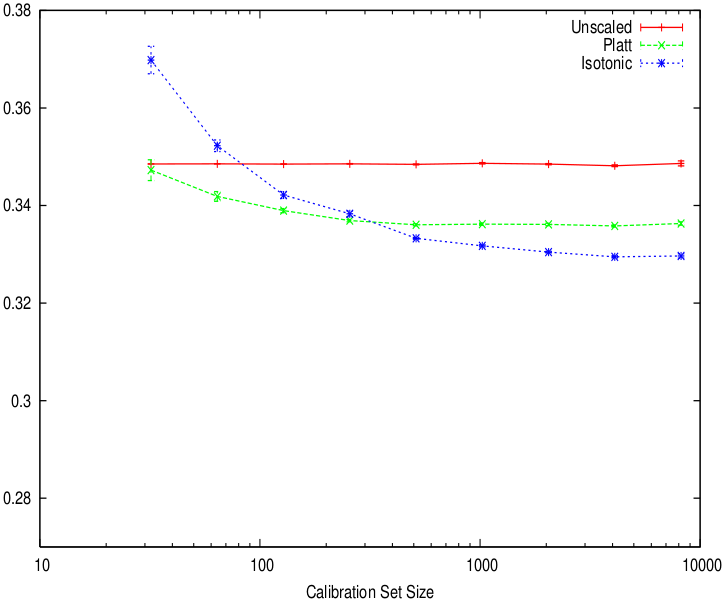
\includegraphics{./calibration_size.png}
\caption{calibration\_size}
\end{figure}

\end{frame}

\begin{frame}{effect of multi-class combination method}

\footnotesize
from Zadrozny and Elkan, 2002

\begin{figure}[htbp]
\centering
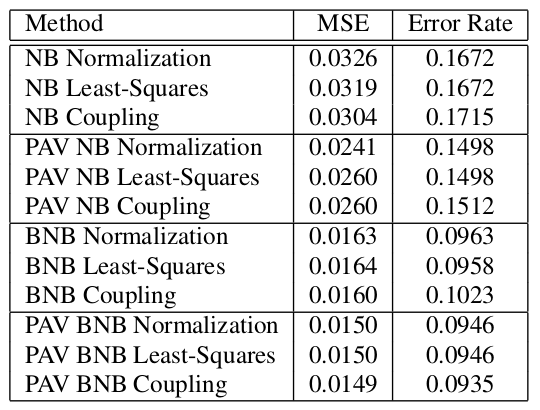
\includegraphics{./multiclass_combination.png}
\caption{combination}
\end{figure}

\end{frame}

\begin{frame}{boosting causes calibration issues}

\footnotesize
from Niculescu-Mizil and Caruana, 2005

\begin{figure}[htbp]
\centering
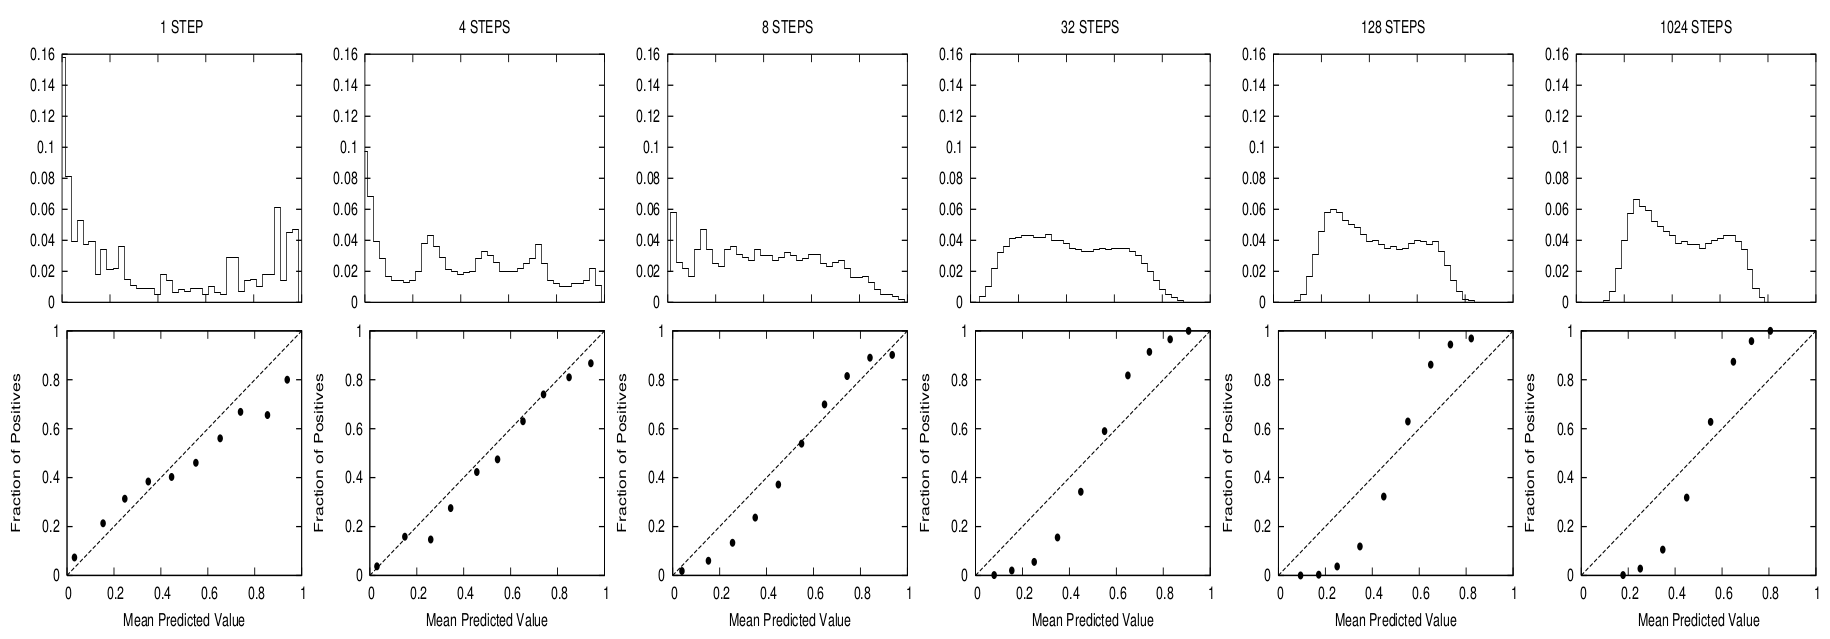
\includegraphics{./boosting.png}
\caption{combination}
\end{figure}

\end{frame}

\section{Conclusion}\label{conclusion}

\begin{frame}{References}

\begin{itemize}
\item
  \textbf{\href{https://www.researchgate.net/publication/28358301_Multivariate_calibration_of_classifier_scores_into_the_probability_space}{Multivariate
  calibration of classifier scores into the probability space}} by
  Martin Gebel
\item
  \textbf{\href{https://www.google.com/url?sa=t\&rct=j\&q=\&esrc=s\&source=web\&cd=4\&cad=rja\&uact=8\&ved=0ahUKEwit7-7h9f7UAhVl6IMKHUPeB2oQFghDMAM\&url=http\%3A\%2F\%2Fwww.cs.cornell.edu\%2Fcourses\%2Fcs678\%2F2007sp\%2FZadroznyElkan.pdf\&usg=AFQjCNEsN8dbe1yXCm7D7qkyrP6HZ6yOxg}{Transforming
  Classifier Scores into Accurate Multiclass Probability Estimates}} by
  Zadrozny and Elkan
\item
  \textbf{\href{http://www.cs.cornell.edu/~caruana/niculescu.scldbst.crc.rev4.pdf}{Obtaining
  Calibrated Probabilities from Boosting}} by Niculescu-Mizil and
  Caruana
\item
  \textbf{\href{https://www.google.com/url?url=http://scholar.google.com/scholar_url\%3Furl\%3Dhttp://machinelearning.wustl.edu/mlpapers/paper_files/icml2005_Niculescu-MizilC05.pdf\%26hl\%3Den\%26sa\%3DX\%26scisig\%3DAAGBfm1wOIFZHQSONJ4oLiHQyqALiSVCng\%26nossl\%3D1\%26oi\%3Dscholarr\&rct=j\&q=\&esrc=s\&sa=X\&ved=0ahUKEwiOotzS9v7UAhXr8YMKHZI8CGsQgAMIJygAMAA\&usg=AFQjCNG3rc7DzDTTox-DD_xm9hwrC5VVQA}{Predicting
  Good Probabilities With Supervised Learning}} by Niculescu-Mizil and
  Caruana
\end{itemize}

\end{frame}

\end{document}
